\section{Markovprozesse und Markov Modelle}

\subsection{Markovketten}
Eine Markovkette ist ein stochastischer Prozess in welchem der nächste Zustand einzig vom gegenwärtigen Zustand abhängt. Diese Eigenschaft ist bekannt als Markov-Eigneschaft \cite{StochasticProcesses}.
\begin{definition}[Markovkette]

    Ein Stochastischer Prozess $\{X_t\}_{t \in T}$, welcher Werte aus einer Menge an Zuständen $S = \{s_1, s_2, \dots, s_n\}$ annehmen kann ist ein Markovprozess, falls gilt
    \begin{equation}
        P(X_{n+1}=s_{n+1} \mid X_{n} = i_{n}, \dots, X_2=i_2, X_1=i_1) = P(X_{n+1}=i_{n+1} \mid X_{n} = i_{n})
    \end{equation}
    Für alle $n \in N_0$ und alle $i_k \in S$ unter der Vorraussetzung, dass alle bedingten Wahrscheinlichkeiten Wohldefiniert sind, also $P(X_{n} = i_{n}, \dots, X_2=i_2, X_1=i_1) > 0$.
\end{definition}

Für solch eine Markovkette definieren wir nun die zwei folgenden Variablen.

\begin{definition}[Startwahrscheinlichkeitsvektor $pi$]

    $\pi$ ist ein Vektor mit Länge $n= |S|$. $\pi_i$ gibt die Wahrscheinlichkeit an, in Zustand $s_i$ zu starten. Also die Wahrscheinlichkeit, dass sich der Prozess in Zeitpunkt $t=0$ in Zustand $s_i$ befindet.
    \begin{equation}
        \pi_i = P(X_0 = s_i)
    \end{equation}
\end{definition}
\begin{definition}[Transitionsmatrix $A$]

    Die Transitionsmatrix $A$ beschreibt die bedingten Wahrscheinlichkeiten, mit denen ein Zustandsübergang geschieht. $a_i(j)$ ist die Wahrscheinlichkeit dass sich der Prozess in Zeitpunkt $t+1$ in Zustand $s_j$ befindet, unter der Bedingung das er sich in Zeitpunk $t$ in Zustand $s_i$ befindet.
    \begin{equation}
        a_{ij} = P(X_{t+1} = s_j \mid X_t = s_i)
    \end{equation}
\end{definition}

Eine Markovkette ist \textbf{zeithomogen} wenn die Transitionswahrscheinlichkeiten $a_{ij}$ unabhängig von der Zeit $t$ sind \cite{HmmIntroduction}.
\begin{align}
    a_{ij} = P(X_{t+1} = s_j \mid X_t = s_i) = P(X_{t} = s_j \mid X_{t-1} = s_i) && 
\end{align}
In dieser Arbeit werden ausschließlich zeithomogene Markovketten betrachtet.

Das Ereignis in irgendeinem Zustand zu starten, so wie das Ereignis von einem gegebenen Zustand in irgendeinen anderen Zustand zu wechseln sind sichere Ereignisse. Somit gelten die Bedingungen, dass die Werte des Startwahrscheinlichkeitsvektors $\pi$ und die Werte der ausgehenden Transitionen für jeden Zustand $A_i$ in Summe jeweils 1 ergeben müssen. Diese Bedingung nennt man \textbf{Reihenstochastizität}
\begin{align}
    \sum_{i = 0}^{N} \pi_i = 1 && \sum_{j = 0}^{N} a_{ij} = 1
\end{align}

Als Beispiel für eine zeitdiskrete homogene Markovkette werden wir die durchschnittliche jährliche Temperatur modellieren. Seien die Zustände des Modells gegeben durch $S=\{H, K\}$, wobei $H$ für heiß und $K$ für kalt steht. Der Startvektor $\pi$ und die Transitionsmatrix $A$ seien gegeben durch
\begin{align}
    \pi = (0.7, 0.3) && 
    A = 
    \begin{bmatrix}
        0.8 & 0.2 \\
        0.4 & 0.6 \\
    \end{bmatrix}
\end{align}

Wir können diese Markovkette anschaulich als gerichteten Transitionsgraphen representieren.

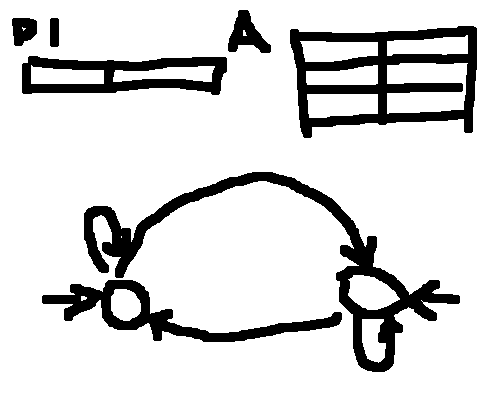
\includegraphics[scale=1.0]{images/Markov_Chain_Example.png}

Mit unserem Temperaturmodell können wir nun zum Beispiel berechnen, was die Wahrscheinlichkeit ist die Temperaturabfolge $O = \{H, K, K, H, H\}$ zu beobachten.
\begin{align*}
    P(O) & = P(O_1 = H) \cdot P(O_2 = K \mid O_1 = H) \cdot P(O_3 = K \mid O_2 = K) \\
    & \cdot P(O_4=H \mid O_3 = K) \cdot P(O_5 = H \mid O_4 = H) \\
    & = \pi_1 \cdot a_{12} \cdot a_{22} \cdot a_{21} \cdot a_{11} \\
    & = 0.7 \cdot 0.2 \cdot 0.6 \cdot 0.4 \cdot 0.8 = 0.02688
\end{align*}

Eine Markovkette gibt uns also die möglichkeit probabilistische Systeme, in denen die Zustände zu den Observationen korrespondieren zu modellieren.

\subsection{Hidden Markov Modelle}
Bei einem Hidden Markov Modell ist die Observationssequenz nicht identisch zur Zustandssequenz, sondern die Observationssymbole sind das Ergebnis einer stochastischen Funktion der Zustände. Die Zustände selbst können wir nicht beobachten denn sie sind "hidden". Ein HMM besteht also aus zwei stochastischen Prozessen. Ein versteckter Prozess, der die Transitionen in Abhängigkeit des vorherigen Zustandes bestimmt und ein zweiter Prozess, der die Observationssymbole in Abhängigkeit des gegenwärtigen Zustandes bestimmt.
Dieser zweite Prozess wird beschrieben durch eine Emissionsmatrix $B$.
\begin{definition}[Emissionsmatrix $B=\{b_j(k)\}$]

    Die Emissionsmatrix $B$ gibt die Wahrscheinlichkeit eines Observationssymbols $v_k$ unter der Bedingung, dass sich der Prozess im gegenwärtigen Zeitpunkt $t$ in Zustand $s_j$ befindet an.
    \begin{align}
        b_j(k) = P(O_t = v_k \mid q_t = S_j) && 1 \leq j \leq N && 1 \leq k \leq M
    \end{align}
\end{definition}

Wie ein solches HMM nun eine Observationssequenz $O$ von Länge $T$ erzeugen kann möchte ich durch folgendes Gedankenexperiment verdeutlichen.

Stellen wir uns einen Raum vor, in dem $N$ Urnen stehen und in welchem sich eine Person befindet. Wir können in diesen Raum nicht hineinsehen. Die Person wird nun insgesamt $T$ Kugeln aus den Urnen ziehen und zurücklegen, wobei sie sich abhängig von einem Zufallsprozess von einer Urne zur nächsten bewegt. Um ethische Bedenken über dieses Gedankenexperiment zu minimieren sei angemerkt, dass der Raum klimatisiert ist und der Person Kakao und Kekse zur Verfügung stehen.
\begin{itemize}
    \item Zunächst wird die initiale Urne anhand des Startwahrscheinlichkeitsvektor $\pi$ ausgewählt.
    \item Dann zieht die Person eine Kugel aus der Urne, notiert deren Farbe als $O_1$ und legt die Kugel zurück.
    \item Danach wird eine neue Urne $q_2 = S_j$ mit Wahrscheinlichkeit $a_{ij} = P(q_2 = S_j \mid q_1 = S_1)$ gewählt. Aus dieser neuen Urne wird die nächste Kugel $O_2$ der Farbe $v_k$ mit Wahrscheinlichkeit $b_j(k)$ gezogen.
\end{itemize}
Diese Prozedur wird so oft wiederholt bis der Zeitpunkt $t=T$ erreicht ist. Wir erhalten somit eine Observationssequenz von Farben $O= \{O_1, O_2, \dots, O_T \}$.
Abbildung \ref{fig:urn_ball_model} zeigt eine Visualisierung dieses Gedankenexperiments für $N=3$

\begin{figure}[h!]
    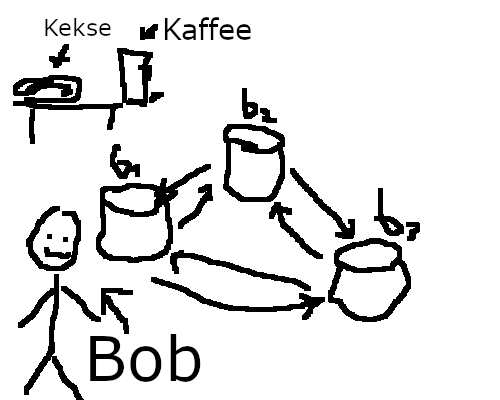
\includegraphics[scale=1.0]{images/Ball_Urn_Model.png}
    \caption{Urn Ball Model}
    \label{fig:urn_ball_model}
\end{figure}

\subsubsection{Die drei Probleme}
Ähnlich wie im Namen der kultigen Hörspielserie über drei junior-Investigatoren aus der kalifornischen Kleinstadt Rocky Beach, präsentieren sich auch im Zusammenhang mit Hidden Markov Modellen drei Fragezeichen. Diese sind allerdings nicht auf einer Visitenkarte anzusiedeln, sondern befinden sich am respektiven Ende folgender Fragen.

- Wie berechnet man die Wahrscheinlichkeit einer Observationssequenz?
- Wie berechnet man die Wahrscheinlichste Zustandssequenz?
- Wie maximiert man die Wahrscheinlichkeit einer Observationssequenz?

\subsubsection{Berechnen der Wahrscheinlichkeit einer Observationssequenz}
Zum Beispiel Was ist die Wahrscheinlichkeit 5 aufeinanderfolgende Jahre mit dicken Baumringen zu beobachten? Formell formuliert $P({L, L, L, L, L} \mid \lambda)$.
Wenn wir die Abfolge der Zustände $Q={q_1, q_2, q_3, q_4, q_5}$ bereits kennen lässt sich $P(O \mid \lambda)$
sehr einfach berechnen. Die Wahrscheinlichkeit ein Symbol $k$ zu beobachten 
unter der Bedingung in Zustand $S_i$ zu sein ist nichts anderes als $B_{i,k}$
Die Wahrscheilichkeit einer Observationssequenz für ein gegebenes Modell und eine gegebene Abfolge von Zuständen ist also
$P(O \mid Q, \lambda) =  \prod_{t=1}^{T} b_{q_t}(O_t)$
Wenn wir die Abfolge der Zustände jedoch nicht kennen gestaltet sich die Berechnung etwas komplizierter.
Die Wahrscheinlichkeit von $P(O \mid \lambda)$ ist equivalent zu der 
Summe der bedingten Wahrscheinlichkeiten aller möglichen Zustandsfolgen.
$P(O \mid \lambda) = \sum_{all Q} P(O \mid Q, \lambda )$
Es ist möglich $P(O \mid \lambda)$ so zu berechnen, jedoch wächst die 
Anzahl der Möglichen Zustandsabfolgen $Q$ exponentiell in Abhängigkeit von der länge der Observationssequenz $T$.
Präzise gesagt gilt $|Q| = 2T \cdot N^T$. Selbst wenn N und T kleine Werte einnehmen
ist die benötigte Rechenleistung untragbar. Für N=5 und T=100
müssten bereits $2 \cdot 100 \cdot 5^{100} \approx 10^{72}$ Berechnungen durchgeführt werden.
Um diese Zahl in Relation zu stellen, $10^{72}$ ist mindestens 3 mal mehr als 1000 und 1000 ist schon ziemlich groß.
Zum Glück gibt es eine effiziente Methode um $P(O \mid \lambda)$ zu berechnen, die Forwärtsvariable.

\subsubsection*{Die Forwärtsvariable}
Sei alpha die Forwärtsvariable folgendermaßen definiert
$\alpha_t(i) = P(O_1 O_2 \dots O_t \wedge q_t = S_i \mid \lambda)$
$\alpha_t(i)$ Beschreibt also die Wahrscheinlichkeit die partielle Observationssequenz
$O_1 O_2 \dots O_t$ zu beobachten und in Zeitpunkt $t$ in in Zustand $i$ zu sein.
$\alpha_t(i)$ kann folgendermaßen induktiv berechnet werden
Für $t=0$ lässt sich $alpha_t(i)$ aus $\pi$ und $B$ berechnen, da noch keine Transition 
stattgefunden hat. 
$\alpha_0(i) = \pi_i \cdot b_i(O_0)$
Für $t>0$ gilt
$\alpha_{t+1}(j) = \left[ \sum_{i=1}^{N} \alpha_t(i) \cdot a_{i,j} \right] \cdot b_j(O_{t+1})$
Der Casus Knacksus, welcher eine effiziente Berechung von $\alpha$ ermöglicht ist die Markov-Eigenschaft.
Diese besagt, dass der Zustand in Zeitpunkt $t+1$ nur vom Zustand in Zeitpunkt $t$ abhängt.
Für jeden Zeitpunkt und jeden Zustand gibt es also genau $N$ Zustände in denen sich
der Prozess zuvor befunden haben kann. Da der Rechenaufwand für jeden Zeitpunkt gleich ist hängt die Komplexität von
$alpha$ mit $N^2 \cdot T$ nur noch linear von $T$ ab und nicht exponentiell wie in dem vorherigen Ansatz.